\section{Ziel}
In diesem Versuch wird mit Hilfe der Doppler-Sonografie die Strömungsgeschwindigkeit verschiedener 
Strömungsröhren untersucht.
Außerdem wird das Strömungsprofil in Abhängigkeit der Strömungsgeschwindigkeit und des Dopplerwinkels bestimmt.




\section[Theorie]{Theorie\footnote[1]{Unter Verwendung von \cite{man:us3}.}}
\subsection{Ultraschall}
Ultraschall befindet sich im Frequenzbereich von \qty{20}{\kilo\hertz} bis \qty{1}{\giga\hertz} und liegt damit oberhalb des für Menschen
hörbaren Bereichs (\qty{16}{\hertz} bis \qty{20}{\kilo\hertz}).

\noindent
Ultraschallwellen können mit Hilfe des piezoelektrischen Effekts erzeugt werden,
bei dem piezoelektrische Kristalle in einem elektrischen Wechselfeld zum Schwingen angeregt werden.
Dabei muss die polare Achse in Richtung des elektrischen Feldes zeigen.
Durch die angeregten Schwingungem werden dann Schallwellen im Ultraschallbereich emittiert.
Sehr hohe Energiedichten des Schalls können im Resonanzfall (Erreger- entspricht der Eigenfrequenz des Kristalls) erreicht werden.
Der Effekt ist reziprok, d.h. treffen Ultraschallwellen auf den Kristall, wird ein elektrisches Wechselfeld erzeugt.
Ein Piezokristall kann somit als Sender und Empfänger genutzt werden.
Trotz des relativ geringen piezoelektrischen Effekts wird häufig Quarz als Kristall benutzt, da es gleichbleibende physikalische 
Eigenschaften besitzt.




\subsection{Der Doppler-Effekt}
Der Doppler-Effekt besagt, dass es Frequenzänderungen gibt, wenn sich Beobachter und Quelle relativ zu einander bewegen.
Sei im Folgenden $\nu_0$ die Frequenz, mit der die Quelle sendet, $v$ die relative Geschwindigkeit zwischen Quelle und Beobachter
und $c$ die Wellengeschwindigkeit im betrachteten Medium.

\noindent
Hat der Beobachter eine feste Position, vergrößert sich die empfangene Frequenz hin zu $\nu_\text{gr}$,
wenn sich die Quelle auf den Beobachter zu bewegt.
Bewegt sie sich vom Beobachter weg, wird die Frequenz kleiner und erreicht den Wert $\nu_\text{kl}$.
Es gilt 
\begin{align}
    \nu_\text{gr/kl} = \frac{\nu_0}{1\mp \frac{v}{c}}.
    \label{eq:gr_kl}
\end{align}

\noindent
Ist hingegen die Quelle fest und der Beobachter bewegt sich, kommt es zu einer höheren Frequenz $\nu_\text{h}$, wenn sich der Beobachter
auf die Quelle zu bewegt, und zu einer niedrigeren Frequenz $\nu_\text{n}$, wenn er sich weg bewegt.
In diesen Fällen gilt
\begin{align}
    \nu_\text{h/n} = \nu_0 \left(1\pm \frac{v}{c}\right).
    \label{eq:h_n}
\end{align}

\noindent
Der Doppler-Effekt findet unter anderem in der Medizin seine Anwendung, um z.B. die Geschwindigkeit von Blutströmungen
zu bestimmen.
Beim Auftreffen einer Ultraschallwelle auf ein bewegtes Objekt, wird die Frequenz um 
\begin{align}
    \Delta \nu = \nu_0 \frac{v}{c} \left(\cos \alpha + \cos \beta\right)
\end{align}
verschoben.
Die beiden Winkel $\alpha$ und $\beta$ sind dabei die Winkel zwischen der Ausbreitungsrichtung (Normale) der einlaufenden bzw.
reflektierten Welle und der Geschwindigkeit $v$ des Objektes an.
Im hier verwendeten Impuls-Echo-Verfahren ist der Sender auch gleichzeitig der Empfänger, sodass sich mit $\alpha = \beta$
die obige Gleichung zu 
\begin{align}
    \Delta \nu = 2 \nu_0 \frac{v}{c} \cos \alpha
    \label{eq:verschiebung}
\end{align}
vereinfacht, vgl. Abbildung \ref{fig:impuls_echo}.

\begin{figure}[H]
    \centering
    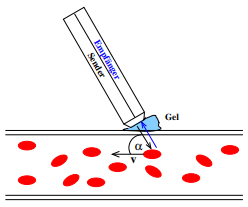
\includegraphics[height = 5 cm]{Abbildungen/impuls_echo.png}
    \caption{Doppler-Sonografie am Beispiel des Impuls-Echo-Verfahrens \cite{man:us3}.}
    \label{fig:impuls_echo}
\end{figure}